\documentclass[11pt]{article}
\usepackage[a4paper,margin=2.2cm]{geometry}
\usepackage{booktabs}
\usepackage{longtable}
\usepackage{graphicx}
\usepackage{float}
\usepackage{hyperref}
\title{Smart-MDT Reproducible Research Evaluation}
\author{Automatically generated evaluation framework}
\date{}

\begin{document}
\maketitle

\section{Overview}
The evaluation contains 7360 benchmark rows, 46
datasets, and 8 methods from
\path{ rust_results_final_freeze_r10_1fbfa30 }. Repeated runs and depths are averaged within each
dataset, and paired comparisons use datasets as independent blocks. Bootstrap
intervals use 10000
resamples, seed 20260718, and a 95.0\% confidence level.

\section{Executive findings}
\begin{itemize}
  \item Best mean accuracy: CALS-MDT
        (0.864820).
  \item Smallest mean tree: CompactExplain
        (11.124 nodes).
  \item Fastest mean fit time: Unary
        (0.047 seconds).
  \item Best mean AXp length: CompactExplain
        (2.721).

  \item For CALS-MDT vs CompactExplain on Accuracy, the right-hand method was lower by 0.0047 (95\% bootstrap CI [-0.0073, -0.0022], raw p=0.001873, Holm-adjusted p=0.01124, paired Cohen's d=-0.523, medium effect).

  \item For SmartCertified vs CALS-MDT on Accuracy, the right-hand method was higher by 0.0052 (95\% bootstrap CI [0.0014, 0.0092], raw p=0.005784, Holm-adjusted p=0.02892, paired Cohen's d=0.385, small effect).

  \item For CALS-MDT vs CompactExplain on Fit time (seconds), the right-hand method was lower by 6.0334 (95\% bootstrap CI [-7.8811, -4.3309], raw p=2.842e-14, Holm-adjusted p=4.263e-13, paired Cohen's d=-0.965, large effect).

  \item For SmartCertified vs CALS-MDT on Fit time (seconds), the right-hand method was higher by 8.1640 (95\% bootstrap CI [5.6094, 11.0623], raw p=5.446e-10, Holm-adjusted p=7.624e-09, paired Cohen's d=0.845, large effect).

  \item For SmartCertified vs CALS-MDT on Tree nodes, the right-hand method was lower by 37.9587 (95\% bootstrap CI [-45.8178, -30.6804], raw p=3.522e-09, Holm-adjusted p=4.576e-08, paired Cohen's d=-1.411, large effect).

  \item For SmartCertified vs CompactExplain on Tree nodes, the right-hand method was lower by 39.5652 (95\% bootstrap CI [-49.0461, -30.9891], raw p=3.52e-09, Holm-adjusted p=4.576e-08, paired Cohen's d=-1.254, large effect).

\end{itemize}

\section{Descriptive statistics}
\begingroup
\small
\setlength{\tabcolsep}{3pt}
\begin{longtable}{llrrrrr}
\caption{Central tendency and dispersion by method and metric.}\label{tab:descriptive-statistics-central}\\
\toprule
Method & Metric & N & Mean & Median & Variance & Std. \\
\midrule
\endfirsthead
\toprule
Method & Metric & N & Mean & Median & Variance & Std. \\
\midrule
\endhead
Unary & Accuracy & 46 & 0.859 & 0.901 & 0.014 & 0.118 \\
Unary & Tree nodes & 46 & 53.235 & 44.050 & 983.710 & 31.364 \\
Unary & Predicate literals & 46 & 26.117 & 21.525 & 245.927 & 15.682 \\
Unary & Mean AXp length & 46 & 3.927 & 3.916 & 1.435 & 1.198 \\
Unary & Fit time (seconds) & 46 & 0.047 & 0.012 & 0.009 & 0.094 \\
Horn & Accuracy & 46 & 0.860 & 0.903 & 0.014 & 0.119 \\
Horn & Tree nodes & 46 & 51.217 & 41.050 & 1061.101 & 32.575 \\
Horn & Predicate literals & 46 & 50.217 & 40.050 & 1061.101 & 32.575 \\
Horn & Mean AXp length & 46 & 5.137 & 5.110 & 2.281 & 1.510 \\
Horn & Fit time (seconds) & 46 & 0.065 & 0.017 & 0.018 & 0.135 \\
AntiHorn & Accuracy & 46 & 0.860 & 0.896 & 0.014 & 0.118 \\
AntiHorn & Tree nodes & 46 & 51.487 & 39.700 & 1089.997 & 33.015 \\
AntiHorn & Predicate literals & 46 & 50.487 & 38.700 & 1089.997 & 33.015 \\
AntiHorn & Mean AXp length & 46 & 5.553 & 5.115 & 4.229 & 2.057 \\
AntiHorn & Fit time (seconds) & 46 & 0.066 & 0.017 & 0.020 & 0.142 \\
Square2CNF & Accuracy & 46 & 0.859 & 0.890 & 0.014 & 0.120 \\
Square2CNF & Tree nodes & 46 & 50.807 & 40.450 & 1112.861 & 33.360 \\
Square2CNF & Predicate literals & 46 & 99.613 & 78.900 & 4451.442 & 66.719 \\
Square2CNF & Mean AXp length & 46 & 6.357 & 6.122 & 4.748 & 2.179 \\
Square2CNF & Fit time (seconds) & 46 & 0.444 & 0.073 & 1.043 & 1.021 \\
Boolean Affine/GF(2) & Accuracy & 46 & 0.854 & 0.881 & 0.014 & 0.119 \\
Boolean Affine/GF(2) & Tree nodes & 46 & 53.126 & 47.300 & 1060.428 & 32.564 \\
Boolean Affine/GF(2) & Predicate literals & 46 & 60.042 & 53.700 & 1238.913 & 35.198 \\
Boolean Affine/GF(2) & Mean AXp length & 46 & 7.897 & 8.185 & 5.437 & 2.332 \\
Boolean Affine/GF(2) & Fit time (seconds) & 46 & 0.162 & 0.031 & 0.120 & 0.346 \\
SmartCertified & Accuracy & 46 & 0.860 & 0.895 & 0.014 & 0.119 \\
SmartCertified & Tree nodes & 46 & 50.689 & 42.300 & 959.944 & 30.983 \\
SmartCertified & Predicate literals & 46 & 30.123 & 26.075 & 294.437 & 17.159 \\
SmartCertified & Mean AXp length & 46 & 4.184 & 4.195 & 1.335 & 1.156 \\
SmartCertified & Fit time (seconds) & 46 & 0.731 & 0.113 & 2.689 & 1.640 \\
CALS-MDT & Accuracy & 46 & 0.865 & 0.896 & 0.014 & 0.118 \\
CALS-MDT & Tree nodes & 46 & 12.730 & 12.800 & 70.748 & 8.411 \\
CALS-MDT & Predicate literals & 46 & 14.936 & 13.600 & 123.817 & 11.127 \\
CALS-MDT & Mean AXp length & 46 & 2.976 & 2.809 & 2.454 & 1.567 \\
CALS-MDT & Fit time (seconds) & 46 & 8.895 & 5.528 & 95.815 & 9.789 \\
CompactExplain & Accuracy & 46 & 0.860 & 0.895 & 0.014 & 0.118 \\
CompactExplain & Tree nodes & 46 & 11.124 & 9.850 & 51.889 & 7.203 \\
CompactExplain & Predicate literals & 46 & 12.786 & 9.550 & 125.144 & 11.187 \\
CompactExplain & Mean AXp length & 46 & 2.721 & 2.553 & 2.867 & 1.693 \\
CompactExplain & Fit time (seconds) & 46 & 2.861 & 1.752 & 15.606 & 3.950 \\
\bottomrule
\end{longtable}
\endgroup

\begingroup
\small
\setlength{\tabcolsep}{3pt}
\begin{longtable}{llrrrr}
\caption{Ranges and 95 percent mean confidence intervals.}\label{tab:descriptive-statistics-intervals}\\
\toprule
Method & Metric & Min. & Max. & 95\% CI lower & 95\% CI upper \\
\midrule
\endfirsthead
\toprule
Method & Metric & Min. & Max. & 95\% CI lower & 95\% CI upper \\
\midrule
\endhead
Unary & Accuracy & 0.543 & 1.000 & 0.824 & 0.894 \\
Unary & Tree nodes & 11.400 & 142.500 & 43.921 & 62.549 \\
Unary & Predicate literals & 5.200 & 70.750 & 21.460 & 30.774 \\
Unary & Mean AXp length & 1.500 & 6.759 & 3.571 & 4.282 \\
Unary & Fit time (seconds) & 0.001 & 0.524 & 0.019 & 0.075 \\
Horn & Accuracy & 0.536 & 1.000 & 0.824 & 0.895 \\
Horn & Tree nodes & 11.400 & 145.700 & 41.544 & 60.891 \\
Horn & Predicate literals & 10.400 & 144.700 & 40.544 & 59.891 \\
Horn & Mean AXp length & 1.594 & 8.976 & 4.689 & 5.586 \\
Horn & Fit time (seconds) & 0.002 & 0.739 & 0.025 & 0.105 \\
AntiHorn & Accuracy & 0.528 & 1.000 & 0.825 & 0.895 \\
AntiHorn & Tree nodes & 11.400 & 138.800 & 41.683 & 61.291 \\
AntiHorn & Predicate literals & 10.400 & 137.800 & 40.683 & 60.291 \\
AntiHorn & Mean AXp length & 1.764 & 10.648 & 4.943 & 6.164 \\
AntiHorn & Fit time (seconds) & 0.002 & 0.802 & 0.024 & 0.109 \\
Square2CNF & Accuracy & 0.535 & 1.000 & 0.824 & 0.895 \\
Square2CNF & Tree nodes & 11.400 & 138.600 & 40.900 & 60.713 \\
Square2CNF & Predicate literals & 20.800 & 275.200 & 79.800 & 119.426 \\
Square2CNF & Mean AXp length & 2.847 & 11.357 & 5.710 & 7.004 \\
Square2CNF & Fit time (seconds) & 0.008 & 4.988 & 0.141 & 0.748 \\
Boolean Affine/GF(2) & Accuracy & 0.537 & 0.997 & 0.818 & 0.889 \\
Boolean Affine/GF(2) & Tree nodes & 11.400 & 144.900 & 43.456 & 62.796 \\
Boolean Affine/GF(2) & Predicate literals & 12.450 & 157.600 & 49.590 & 70.495 \\
Boolean Affine/GF(2) & Mean AXp length & 3.516 & 13.809 & 7.205 & 8.590 \\
Boolean Affine/GF(2) & Fit time (seconds) & 0.005 & 1.754 & 0.060 & 0.265 \\
SmartCertified & Accuracy & 0.544 & 1.000 & 0.824 & 0.895 \\
SmartCertified & Tree nodes & 11.400 & 141.500 & 41.488 & 59.890 \\
SmartCertified & Predicate literals & 5.200 & 76.750 & 25.027 & 35.218 \\
SmartCertified & Mean AXp length & 1.920 & 7.459 & 3.841 & 4.527 \\
SmartCertified & Fit time (seconds) & 0.008 & 8.272 & 0.244 & 1.218 \\
CALS-MDT & Accuracy & 0.537 & 0.999 & 0.830 & 0.900 \\
CALS-MDT & Tree nodes & 1.000 & 42.400 & 10.233 & 15.228 \\
CALS-MDT & Predicate literals & 0.000 & 51.050 & 11.631 & 18.240 \\
CALS-MDT & Mean AXp length & 0.000 & 8.273 & 2.511 & 3.442 \\
CALS-MDT & Fit time (seconds) & 0.340 & 44.199 & 5.988 & 11.801 \\
CompactExplain & Accuracy & 0.539 & 1.000 & 0.825 & 0.895 \\
CompactExplain & Tree nodes & 1.000 & 32.500 & 8.985 & 13.263 \\
CompactExplain & Predicate literals & 0.000 & 58.950 & 9.464 & 16.108 \\
CompactExplain & Mean AXp length & 0.000 & 9.274 & 2.219 & 3.224 \\
CompactExplain & Fit time (seconds) & 0.121 & 19.187 & 1.688 & 4.034 \\
\bottomrule
\end{longtable}
\endgroup


\section{Pairwise significance}
Positive differences and effect sizes indicate that the right-hand method has
the larger metric value. Accuracy is maximized; nodes, literals, AXp length,
and runtime are minimized. Holm-adjusted p-values control family-wise error
across the configured tests.
\begin{table}[htbp]
\centering
\caption{Paired Wilcoxon tests with Holm-adjusted p-values and bootstrap confidence intervals.}
\label{tab:significance-tests}
\resizebox{\textwidth}{!}{%
\begin{tabular}{llrrrrrrr}
\toprule
Comparison & Metric & Pairs & Mean diff. & Wilcoxon W & p-value & Holm p-value & Bootstrap lower & Bootstrap upper \\
\midrule
SmartCertified vs CALS-MDT & Accuracy & 46 & 0.005 & 273.000 & 0.006 & 0.029 & 0.001 & 0.009 \\
SmartCertified vs CALS-MDT & Tree nodes & 46 & -37.959 & 0.000 & 0.000 & 0.000 & -45.818 & -30.680 \\
SmartCertified vs CALS-MDT & Predicate literals & 46 & -15.187 & 72.000 & 0.000 & 0.000 & -19.710 & -10.872 \\
SmartCertified vs CALS-MDT & Mean AXp length & 46 & -1.207 & 146.000 & 0.000 & 0.000 & -1.635 & -0.768 \\
SmartCertified vs CALS-MDT & Fit time (seconds) & 46 & 8.164 & 46.000 & 0.000 & 0.000 & 5.609 & 11.062 \\
SmartCertified vs CompactExplain & Accuracy & 46 & 0.001 & 525.000 & 0.871 & 0.871 & -0.004 & 0.005 \\
SmartCertified vs CompactExplain & Tree nodes & 46 & -39.565 & 0.000 & 0.000 & 0.000 & -49.046 & -30.989 \\
SmartCertified vs CompactExplain & Predicate literals & 46 & -17.337 & 95.000 & 0.000 & 0.000 & -23.148 & -11.750 \\
SmartCertified vs CompactExplain & Mean AXp length & 46 & -1.463 & 139.000 & 0.000 & 0.000 & -1.962 & -0.957 \\
SmartCertified vs CompactExplain & Fit time (seconds) & 46 & 2.131 & 122.000 & 0.000 & 0.000 & 1.132 & 3.300 \\
CALS-MDT vs CompactExplain & Accuracy & 46 & -0.005 & 242.000 & 0.002 & 0.011 & -0.007 & -0.002 \\
CALS-MDT vs CompactExplain & Tree nodes & 46 & -1.607 & 443.500 & 0.404 & 0.807 & -3.511 & 0.102 \\
CALS-MDT vs CompactExplain & Predicate literals & 46 & -2.150 & 382.500 & 0.128 & 0.383 & -4.110 & -0.317 \\
CALS-MDT vs CompactExplain & Mean AXp length & 46 & -0.255 & 328.000 & 0.032 & 0.130 & -0.543 & 0.057 \\
CALS-MDT vs CompactExplain & Fit time (seconds) & 46 & -6.033 & 0.000 & 0.000 & 0.000 & -7.881 & -4.331 \\
\bottomrule
\end{tabular}%
}
\end{table}

\begin{table}[htbp]
\centering
\caption{Cliff's delta and paired Cohen's d effect sizes.}
\label{tab:significance-effects}
\resizebox{\textwidth}{!}{%
\begin{tabular}{llrlrl}
\toprule
Comparison & Metric & Cliff's delta & Cliff magnitude & Cohen's d & d magnitude \\
\midrule
SmartCertified vs CALS-MDT & Accuracy & 0.034 & negligible & 0.385 & small \\
SmartCertified vs CALS-MDT & Tree nodes & -0.863 & large & -1.411 & large \\
SmartCertified vs CALS-MDT & Predicate literals & -0.552 & large & -0.978 & large \\
SmartCertified vs CALS-MDT & Mean AXp length & -0.491 & large & -0.803 & large \\
SmartCertified vs CALS-MDT & Fit time (seconds) & 0.871 & large & 0.845 & large \\
SmartCertified vs CompactExplain & Accuracy & 0.000 & negligible & 0.041 & negligible \\
SmartCertified vs CompactExplain & Tree nodes & -0.910 & large & -1.254 & large \\
SmartCertified vs CompactExplain & Predicate literals & -0.647 & large & -0.866 & large \\
SmartCertified vs CompactExplain & Mean AXp length & -0.617 & large & -0.821 & large \\
SmartCertified vs CompactExplain & Fit time (seconds) & 0.698 & large & 0.568 & medium \\
CALS-MDT vs CompactExplain & Accuracy & -0.032 & negligible & -0.523 & medium \\
CALS-MDT vs CompactExplain & Tree nodes & -0.105 & negligible & -0.253 & small \\
CALS-MDT vs CompactExplain & Predicate literals & -0.138 & negligible & -0.328 & small \\
CALS-MDT vs CompactExplain & Mean AXp length & -0.125 & negligible & -0.243 & small \\
CALS-MDT vs CompactExplain & Fit time (seconds) & -0.496 & large & -0.965 & large \\
\bottomrule
\end{tabular}%
}
\end{table}


\section{Dataset analysis}
The Nemenyi critical difference for average accuracy ranks is
1.548.
\begingroup
\small
\setlength{\tabcolsep}{3pt}
\begin{longtable}{llrrrr}
\caption{Best method and associated metrics for every dataset.}\label{tab:dataset-summary}\\
\toprule
Dataset & Best method & Accuracy & Nodes & AXp & Runtime (s) \\
\midrule
\endfirsthead
\toprule
Dataset & Best method & Accuracy & Nodes & AXp & Runtime (s) \\
\midrule
\endhead
HTRU\_2-bin & Unary & 0.976 & 111.900 & 2.277 & 0.082 \\
IndiansDiabetes-bin & CALS-MDT & 0.741 & 14.100 & 3.871 & 22.738 \\
Statlog\_satellite-bin & CALS-MDT & 0.960 & 24.100 & 4.166 & 3.862 \\
adult\_discretized & Boolean Affine/GF(2) & 0.853 & 118.500 & 7.868 & 1.169 \\
anneal & CALS-MDT & 0.856 & 12.800 & 5.032 & 1.019 \\
audiology & Horn & 0.955 & 14.200 & 3.398 & 0.002 \\
australian-credit & CompactExplain & 0.864 & 5.800 & 1.358 & 1.582 \\
balance-scale-bin & CALS-MDT & 0.917 & 1.700 & 0.116 & 10.404 \\
bank\_conv-bin & Unary & 0.902 & 93.100 & 6.442 & 0.071 \\
banknote-bin & Square2CNF & 0.990 & 30.200 & 5.054 & 0.052 \\
biodeg-bin & CALS-MDT & 0.818 & 20.300 & 5.128 & 21.699 \\
breast-cancer-un & CALS-MDT & 0.943 & 5.800 & 2.530 & 9.736 \\
breast-wisconsin & CALS-MDT & 0.950 & 7.000 & 2.704 & 7.035 \\
car-un & Square2CNF & 0.968 & 31.200 & 3.607 & 0.071 \\
car\_evaluation-bin & SmartCertified & 0.942 & 38.400 & 2.585 & 0.014 \\
compas\_discretized & Unary & 0.671 & 107.100 & 4.325 & 0.011 \\
diabetes & Unary & 0.744 & 83.500 & 5.342 & 0.012 \\
forest-fires-un & SmartCertified & 0.544 & 18.500 & 4.583 & 0.138 \\
german-credit & CompactExplain & 0.728 & 12.900 & 2.929 & 4.282 \\
heart-cleveland & CALS-MDT & 0.776 & 7.000 & 2.791 & 12.669 \\
hepatitis & CALS-MDT & 0.856 & 2.600 & 1.020 & 5.111 \\
hypothyroid & Unary & 0.980 & 42.300 & 1.932 & 0.011 \\
ionosphere & CALS-MDT & 0.878 & 5.900 & 2.174 & 2.077 \\
kr-vs-kp & CompactExplain & 0.988 & 28.500 & 4.228 & 4.464 \\
letter & Square2CNF & 0.989 & 72.900 & 6.225 & 1.480 \\
letter\_recognition-bin & AntiHorn & 0.996 & 61.600 & 6.158 & 0.350 \\
lymph & SmartCertified & 0.819 & 21.700 & 3.675 & 0.011 \\
magic04-bin & Square2CNF & 0.837 & 138.600 & 7.620 & 3.381 \\
messidor-bin & CompactExplain & 0.643 & 9.400 & 2.548 & 0.162 \\
mushroom & CompactExplain & 1.000 & 9.800 & 4.938 & 1.877 \\
pendigits & SmartCertified & 0.996 & 43.700 & 3.727 & 0.704 \\
primary-tumor & CompactExplain & 0.815 & 11.100 & 1.840 & 1.785 \\
segment & Boolean Affine/GF(2) & 0.997 & 11.400 & 5.758 & 0.020 \\
seismic\_bumps-bin & CompactExplain & 0.922 & 1.000 & 0.000 & 3.537 \\
soybean & CALS-MDT & 0.942 & 12.800 & 4.043 & 11.055 \\
splice-1 & Unary & 0.955 & 74.300 & 4.291 & 0.058 \\
taiwan\_binarised & CALS-MDT & 0.821 & 11.700 & 1.810 & 5.873 \\
tic-tac-toe & Horn & 0.918 & 47.200 & 4.726 & 0.006 \\
titanic-un & CALS-MDT & 0.819 & 16.300 & 2.969 & 8.384 \\
vehicle & SmartCertified & 0.946 & 36.600 & 3.956 & 0.092 \\
vote & CompactExplain & 0.945 & 6.200 & 1.923 & 1.516 \\
wine1-un & AntiHorn & 0.708 & 13.000 & 10.202 & 0.018 \\
wine2-un & AntiHorn & 0.664 & 15.700 & 10.425 & 0.018 \\
wine3-un & CALS-MDT & 0.751 & 3.800 & 4.053 & 0.359 \\
winequality-red-bin & CompactExplain & 0.994 & 1.000 & 0.000 & 0.379 \\
yeast & CALS-MDT & 0.717 & 21.400 & 3.888 & 2.067 \\
\bottomrule
\end{longtable}
\endgroup

\begin{table}[htbp]
\centering
\caption{Dataset wins and average accuracy ranks. The critical difference uses a two-sided Nemenyi comparison at alpha 0.05.}
\label{tab:dataset-ranks}
\resizebox{\textwidth}{!}{%
\begin{tabular}{lrrr}
\toprule
Method & Wins & Average rank & Critical difference \\
\midrule
CALS-MDT & 15 & 3.120 & 1.548 \\
Unary & 6 & 4.130 & 1.548 \\
SmartCertified & 5 & 4.228 & 1.548 \\
Horn & 2 & 4.370 & 1.548 \\
CompactExplain & 9 & 4.522 & 1.548 \\
Square2CNF & 4 & 4.598 & 1.548 \\
AntiHorn & 3 & 4.685 & 1.548 \\
Boolean Affine/GF(2) & 2 & 6.348 & 1.548 \\
\bottomrule
\end{tabular}%
}
\end{table}


\begin{figure}[H]
\centering
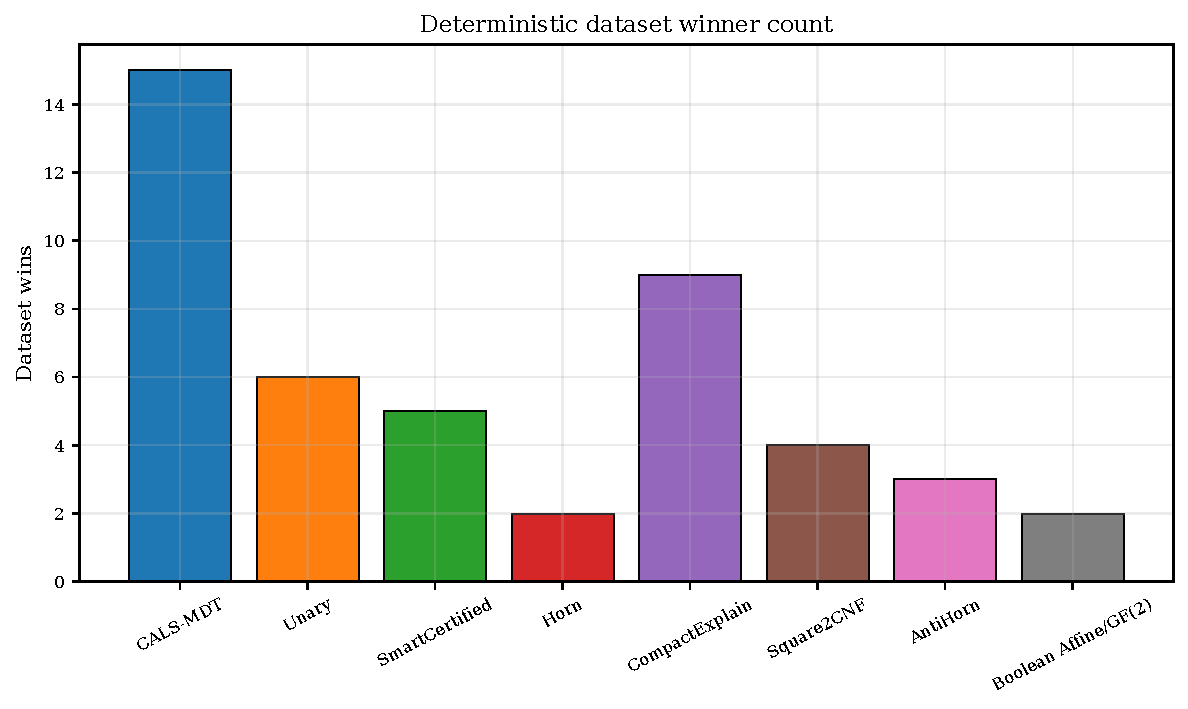
\includegraphics[width=0.78\textwidth]{../figures/dataset_win_histogram.pdf}
\caption{Dataset winner counts.}
\end{figure}

\begin{figure}[H]
\centering
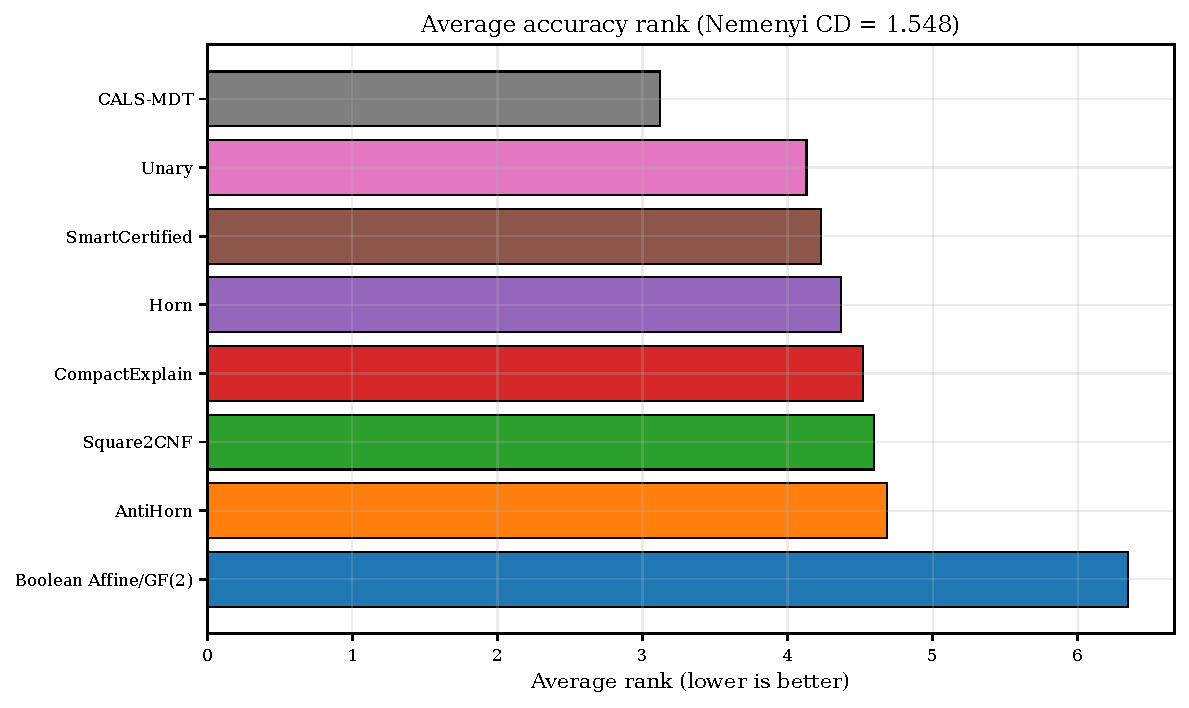
\includegraphics[width=0.78\textwidth]{../figures/average_rank.pdf}
\caption{Average dataset accuracy ranks.}
\end{figure}

\section{Performance and explanation figures}

\begin{figure}[H]
\centering
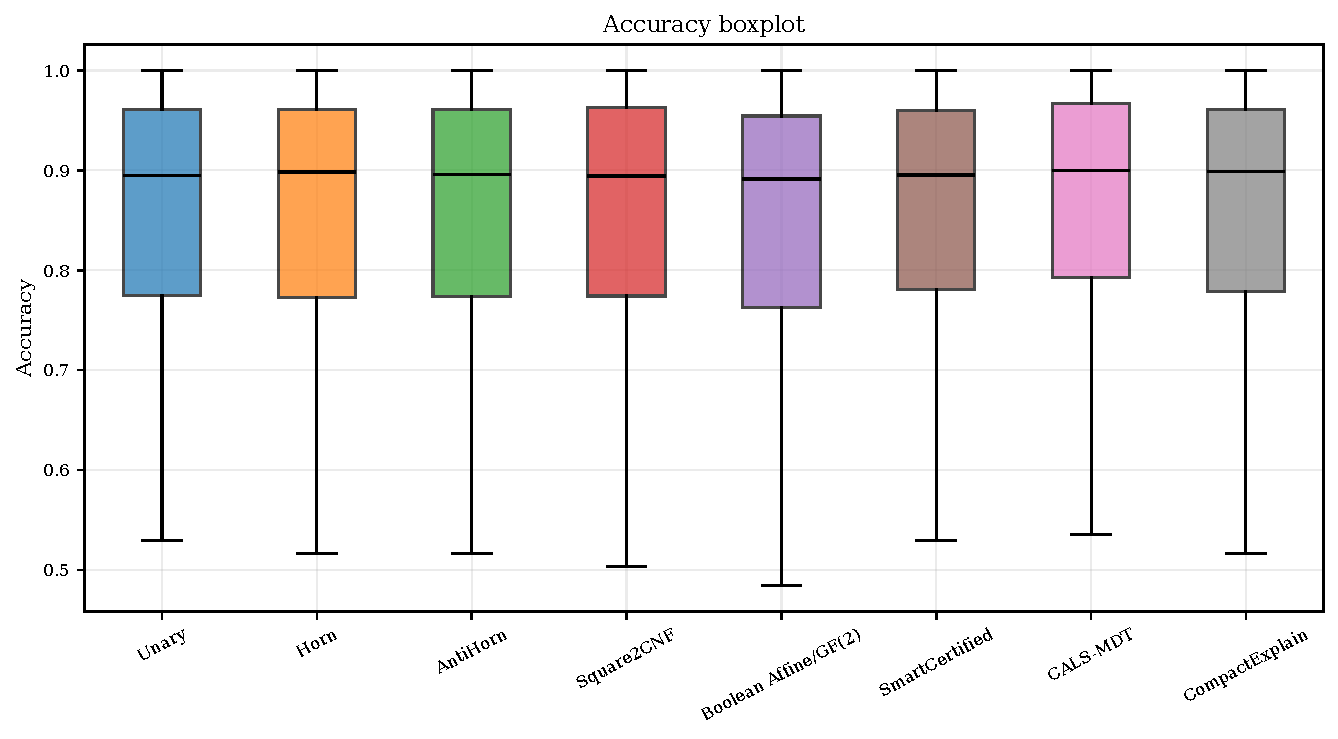
\includegraphics[width=0.82\textwidth]{../figures/accuracy_boxplot.pdf}
\caption{ Accuracy boxplot. }
\end{figure}

\begin{figure}[H]
\centering
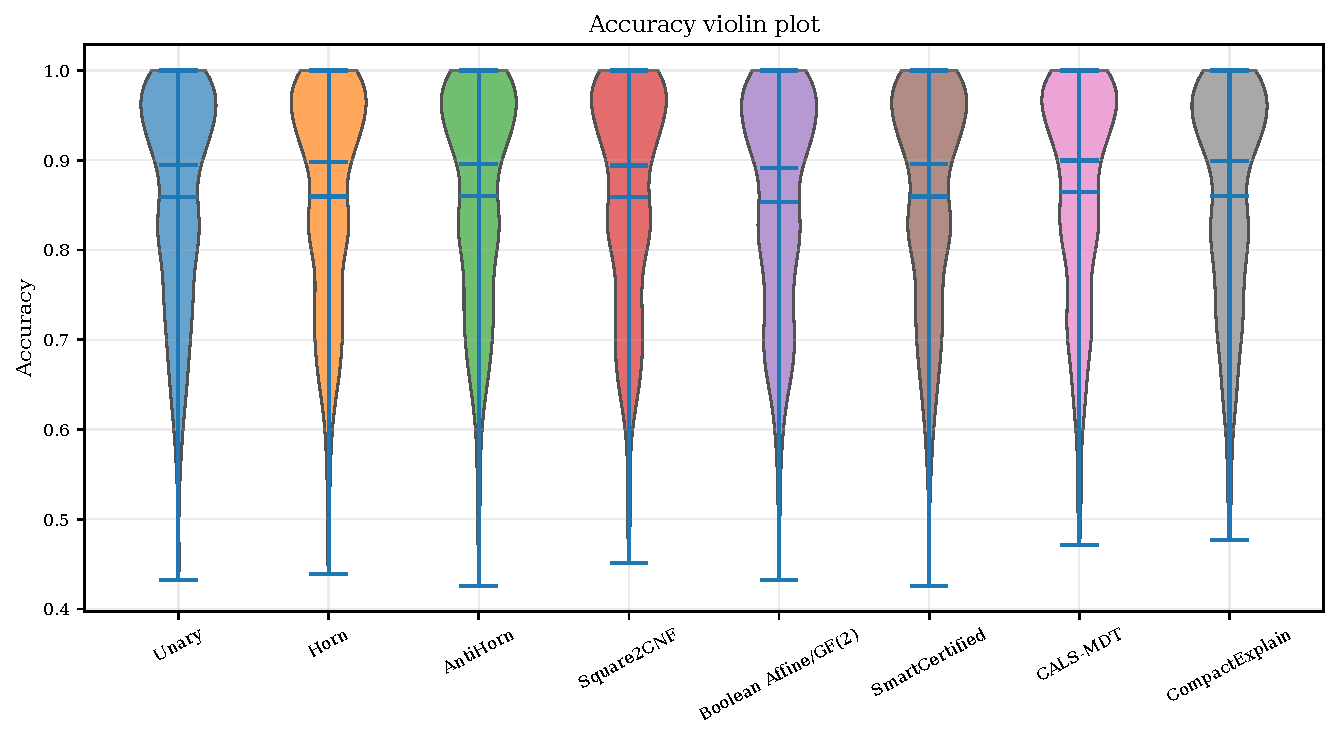
\includegraphics[width=0.82\textwidth]{../figures/accuracy_violin.pdf}
\caption{ Accuracy violin plot. }
\end{figure}

\begin{figure}[H]
\centering
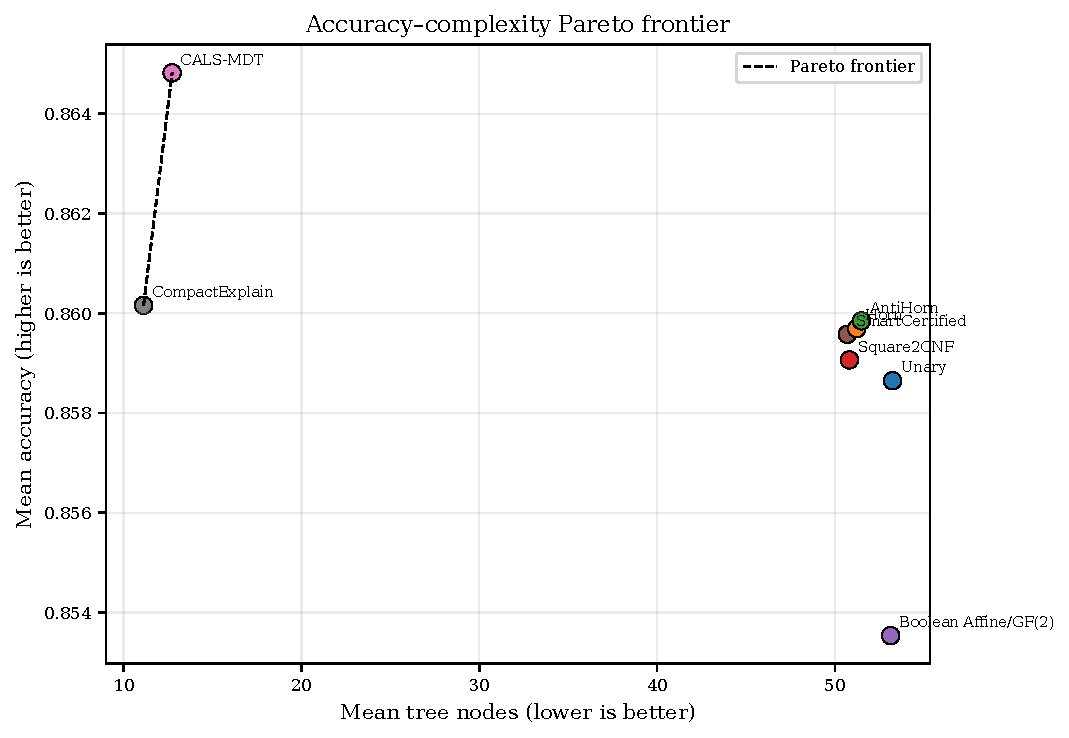
\includegraphics[width=0.82\textwidth]{../figures/pareto.pdf}
\caption{ Accuracy--complexity Pareto frontier. }
\end{figure}

\begin{figure}[H]
\centering
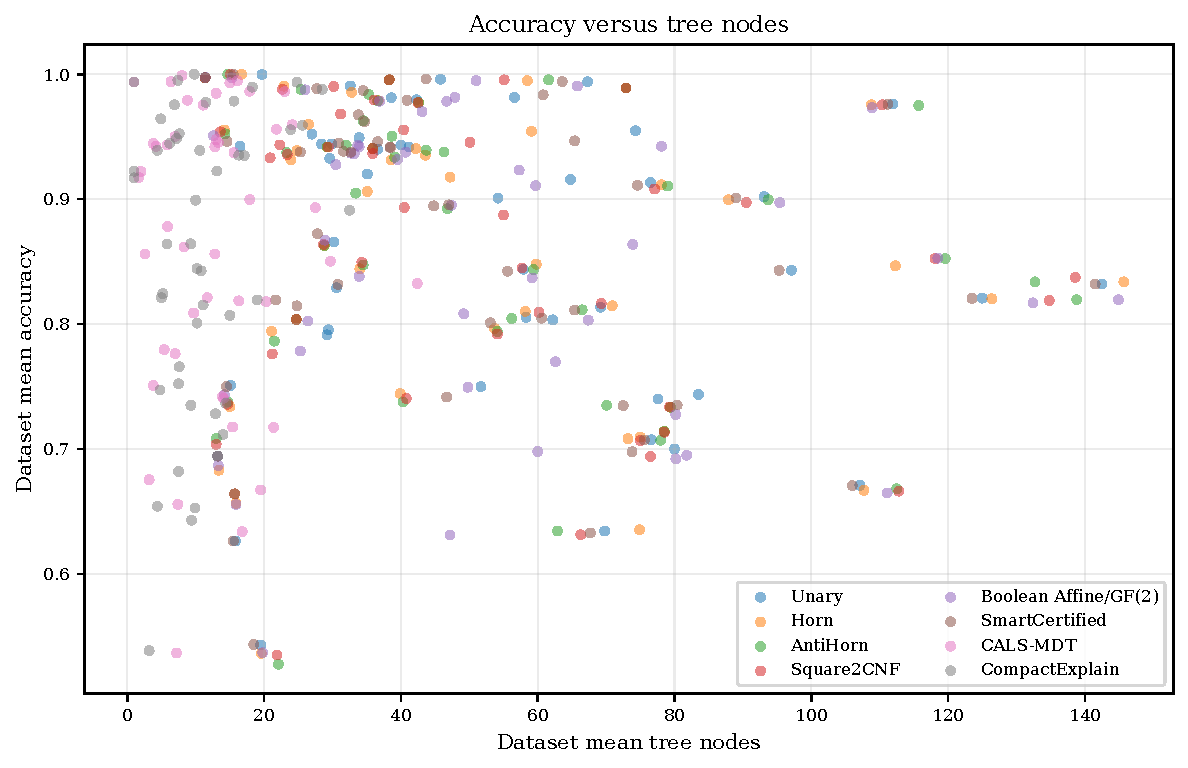
\includegraphics[width=0.82\textwidth]{../figures/accuracy_vs_nodes.pdf}
\caption{ Accuracy versus tree nodes. }
\end{figure}

\begin{figure}[H]
\centering
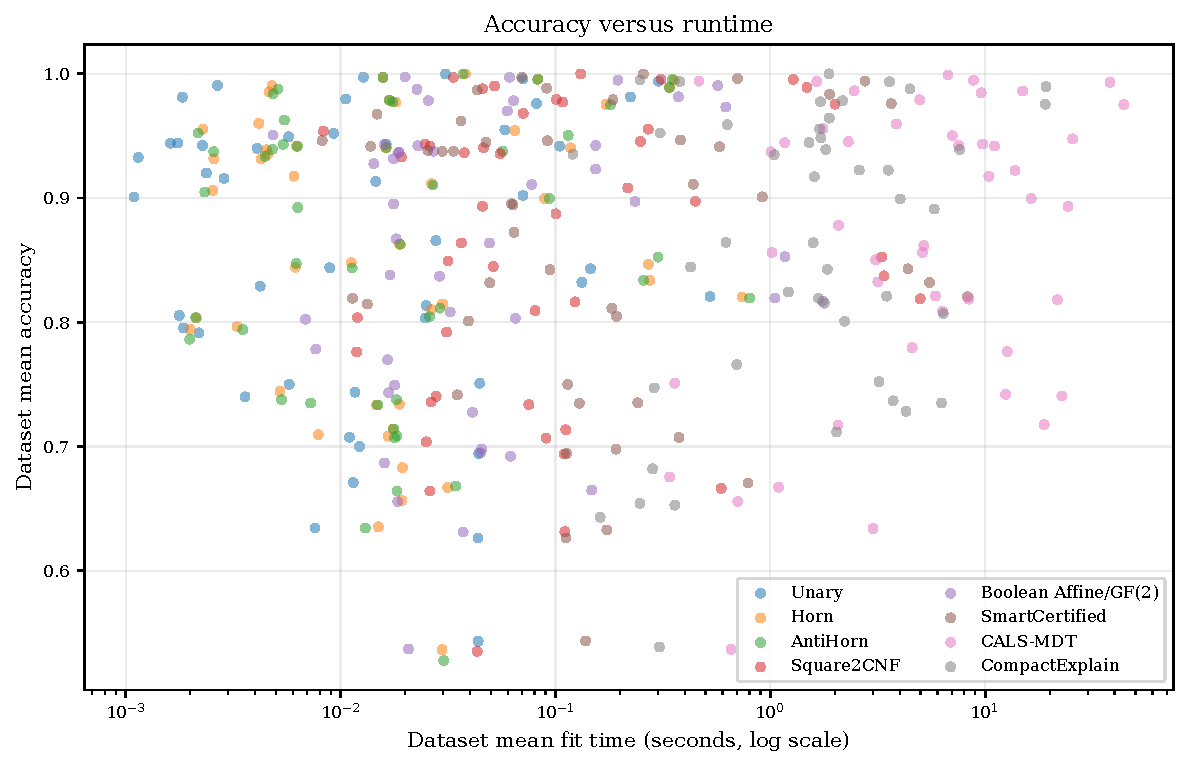
\includegraphics[width=0.82\textwidth]{../figures/accuracy_vs_runtime.pdf}
\caption{ Accuracy versus runtime. }
\end{figure}

\begin{figure}[H]
\centering
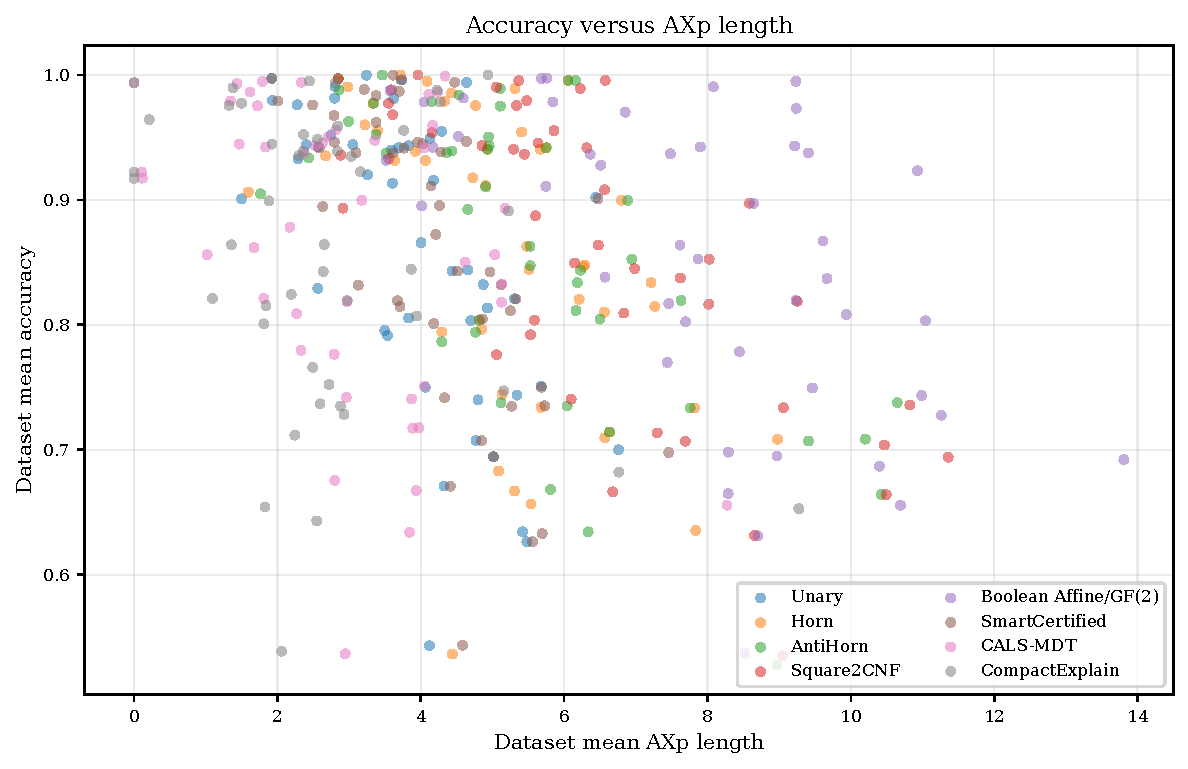
\includegraphics[width=0.82\textwidth]{../figures/accuracy_vs_axp.pdf}
\caption{ Accuracy versus AXp length. }
\end{figure}

\begin{figure}[H]
\centering
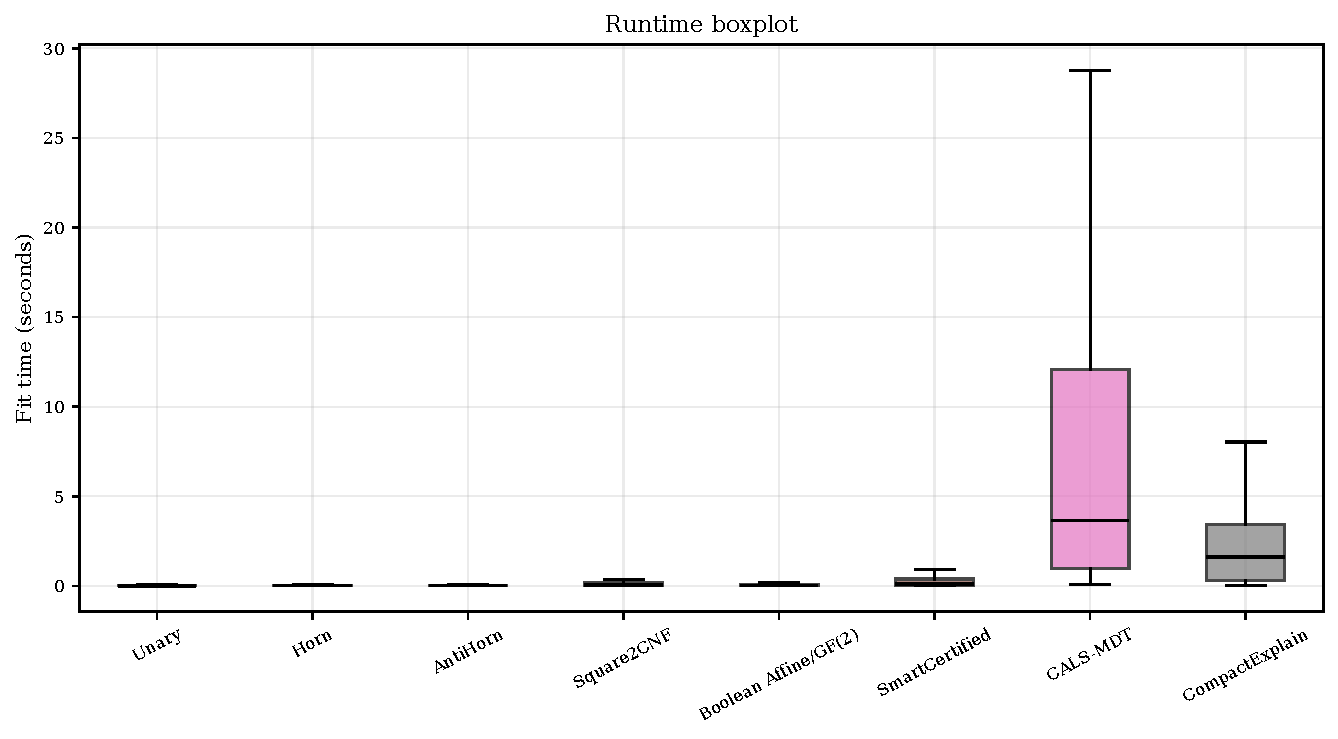
\includegraphics[width=0.82\textwidth]{../figures/runtime_boxplot.pdf}
\caption{ Runtime boxplot. }
\end{figure}

\begin{figure}[H]
\centering
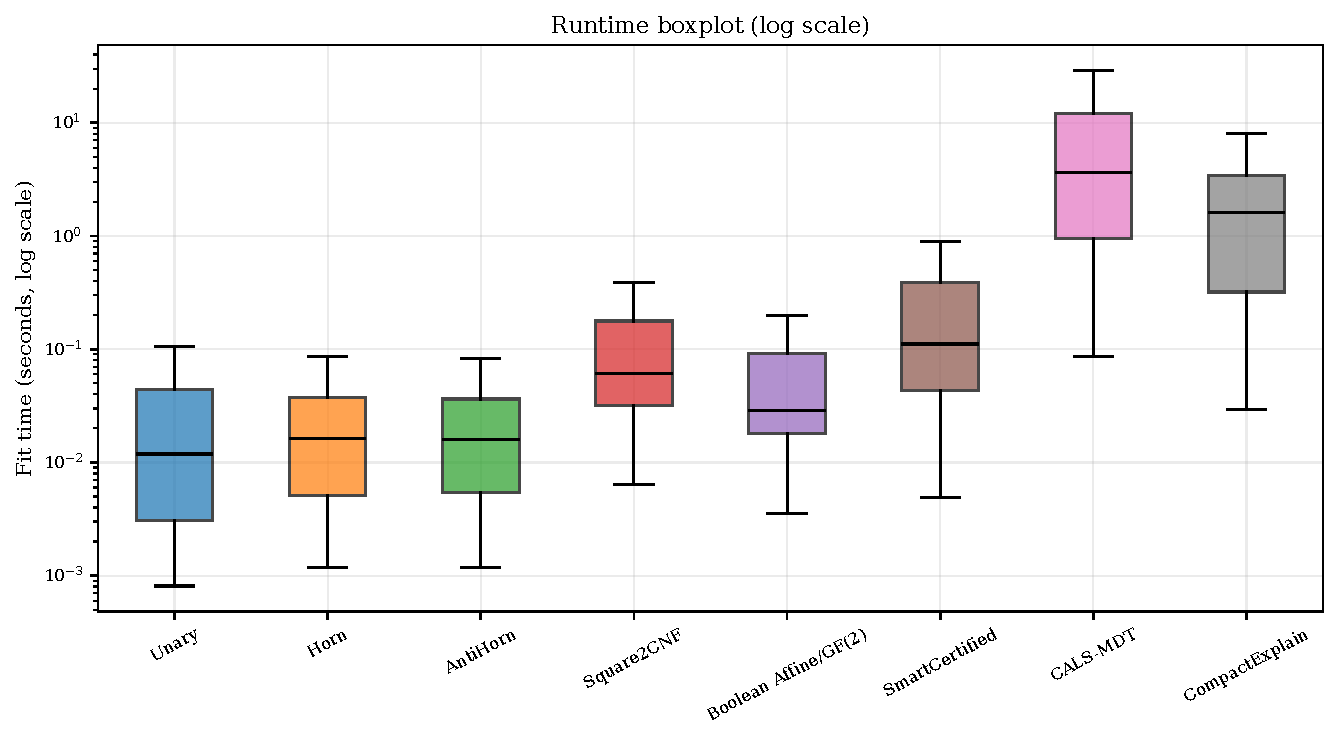
\includegraphics[width=0.82\textwidth]{../figures/runtime_log_boxplot.pdf}
\caption{ Runtime boxplot on a logarithmic scale. }
\end{figure}

\begin{figure}[H]
\centering
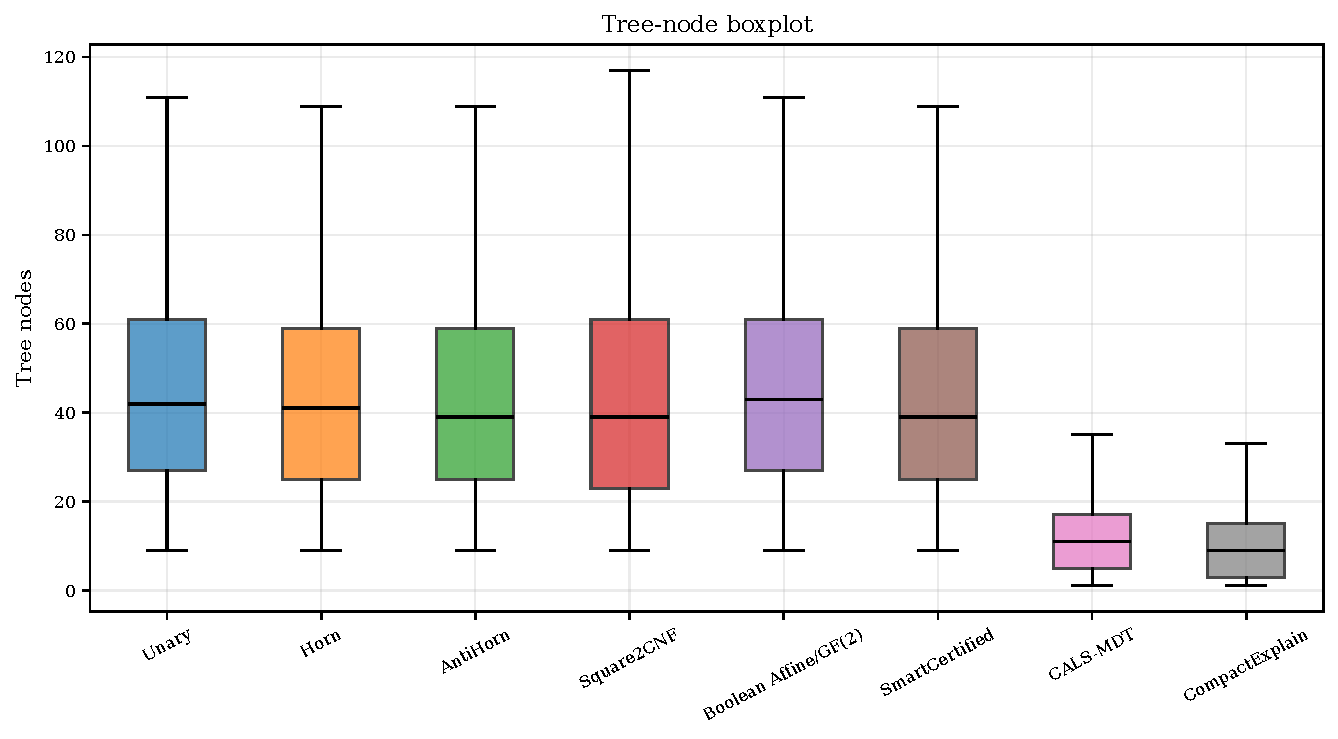
\includegraphics[width=0.82\textwidth]{../figures/nodes_boxplot.pdf}
\caption{ Tree-node boxplot. }
\end{figure}

\begin{figure}[H]
\centering
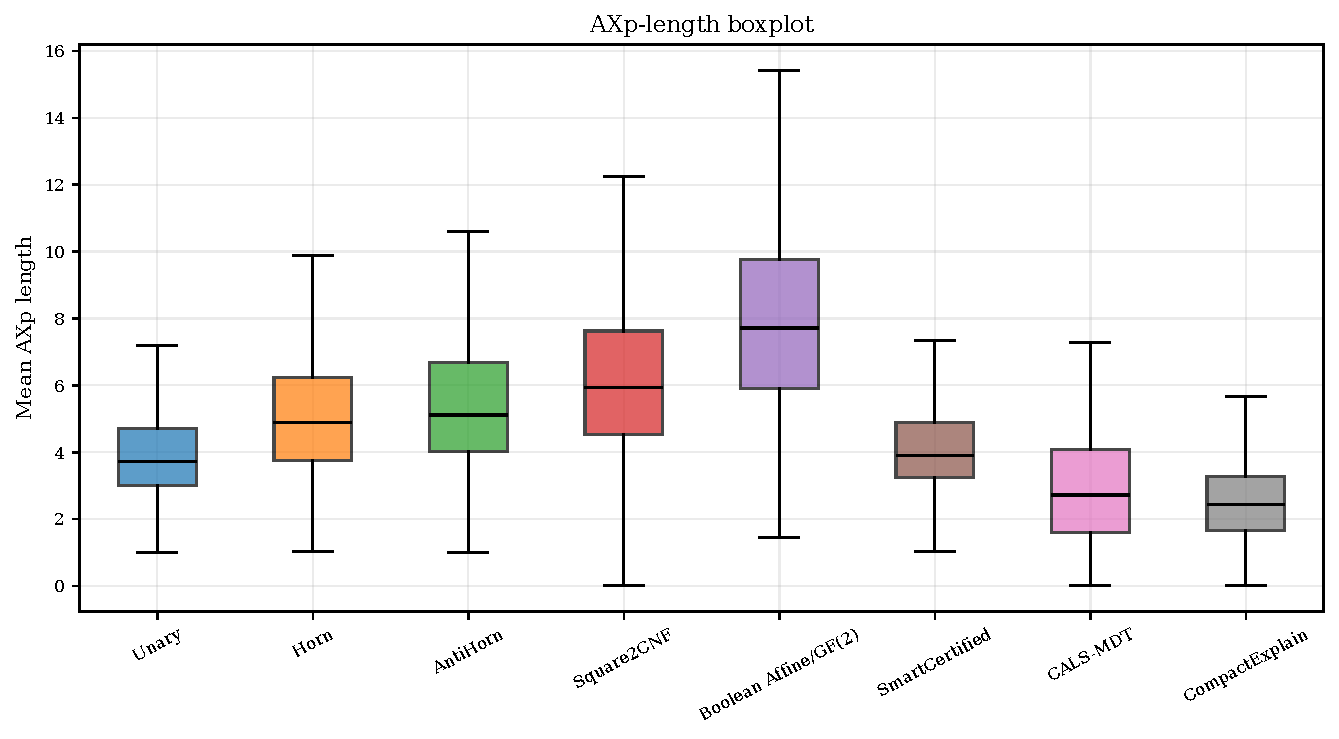
\includegraphics[width=0.82\textwidth]{../figures/axp_boxplot.pdf}
\caption{ AXp-length boxplot. }
\end{figure}

\begin{figure}[H]
\centering
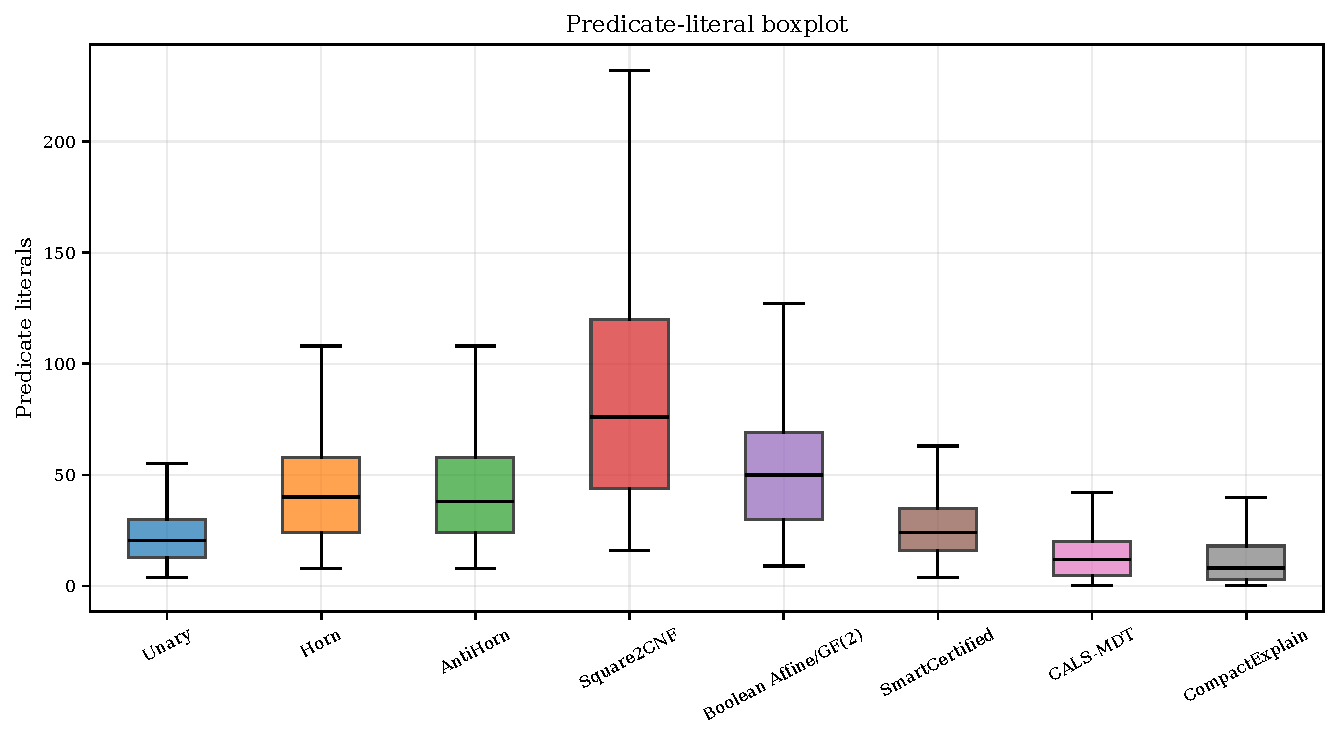
\includegraphics[width=0.82\textwidth]{../figures/predicate_literals_boxplot.pdf}
\caption{ Predicate-literal boxplot. }
\end{figure}


\section{Certification}
\begin{table}[htbp]
\centering
\caption{Certification and data-integrity audit.}
\label{tab:certification-summary}
\resizebox{\textwidth}{!}{%
\begin{tabular}{lrrrrl}
\toprule
Audit item & Count & Denominator & Percentage & evidence\_available & status \\
\midrule
datasets & 46 & 46 & 100.000 & 1 & pass \\
rows & 7360 & 7360 & 100.000 & 1 & pass \\
theorem\_certified\_rows & 7360 & 7360 & 100.000 & 1 & pass \\
empirical\_rows & 0 & 7360 & 0.000 & 1 & pass \\
forbidden\_predicates & 0 & 7360 & 0.000 & 1 & pass \\
feature\_label\_leakage & 0 & 46 & 0.000 & 1 & pass \\
path\_violations & 0 & 7360 & 0.000 & 1 & pass \\
cached\_subtree\_violations & 0 & 7360 & 0.000 & 1 & pass \\
empirical\_fallbacks & 0 & 7360 & 0.000 & 1 & pass \\
axp\_evidence\_violations & 0 & 7360 & 0.000 & 1 & pass \\
full\_row\_axp\_violations & 0 & 7360 & 0.000 & 1 & pass \\
skipped\_datasets & 0 & 46 & 0.000 & 1 & pass \\
\bottomrule
\end{tabular}%
}
\end{table}

\begin{figure}[H]
\centering
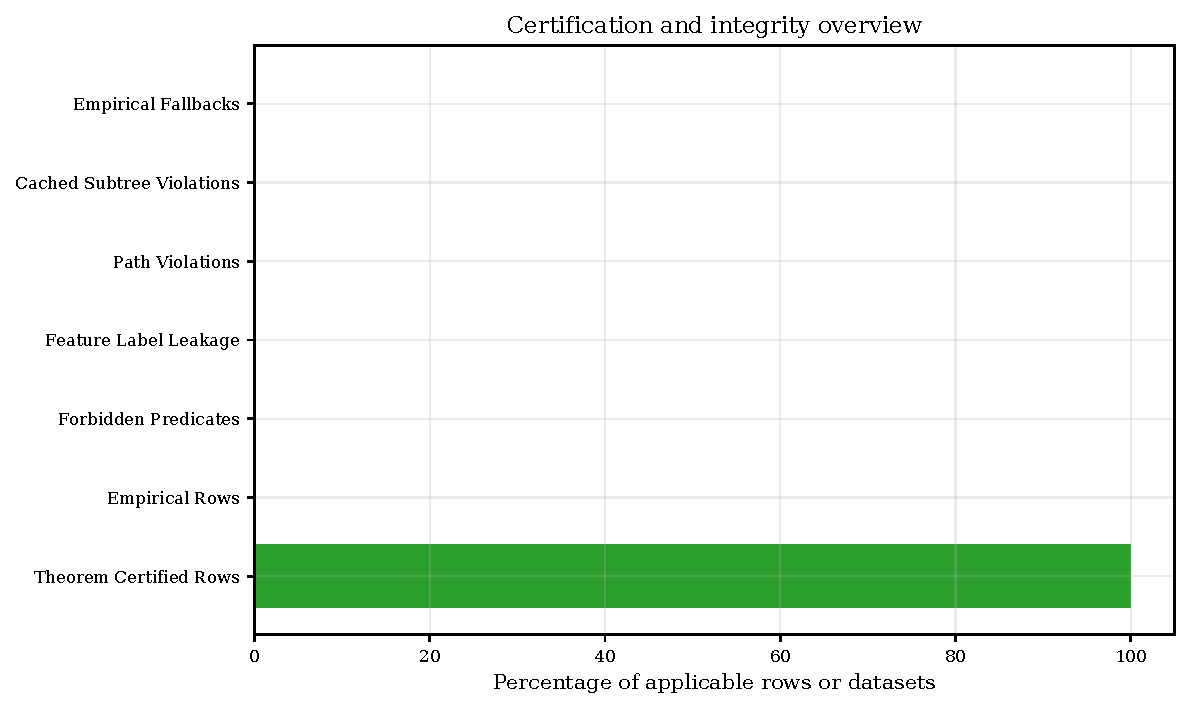
\includegraphics[width=0.82\textwidth]{../figures/certification_overview.pdf}
\caption{Certification and integrity audit.}
\end{figure}

\section{Benchmark warnings}
The warning summary contains 11 grouped records. The
machine-readable table is available as
\texttt{../tables/warnings\_summary.csv}.
\begin{figure}[H]
\centering
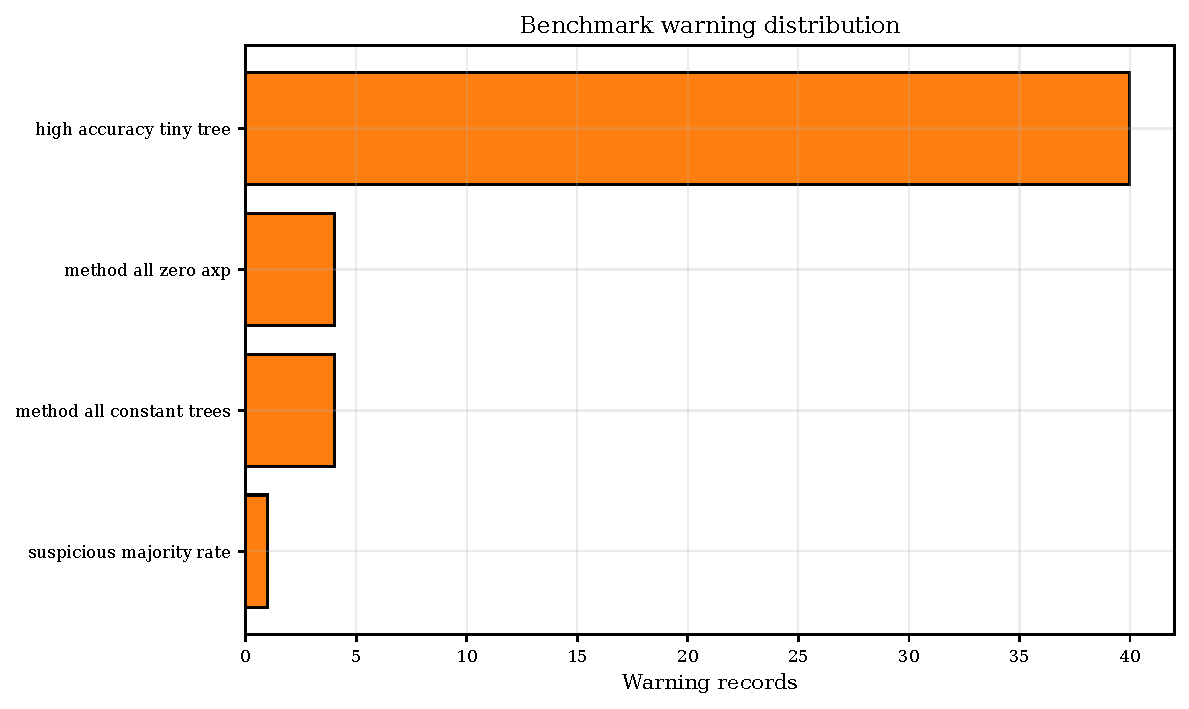
\includegraphics[width=0.82\textwidth]{../figures/warning_distribution.pdf}
\caption{Benchmark warning distribution.}
\end{figure}

\section{Search analysis}
\begin{table}[htbp]
\centering
\caption{Search-selection diagnostics.}
\label{tab:search-selection}
\resizebox{\textwidth}{!}{%
\begin{tabular}{lrrrrr}
\toprule
Method & Rows & Greedy nodes & Lookahead nodes & B\&B active & B\&B avoided \\
\midrule
Unary & 920 & 0.000 & 0.000 & 0.000 & 0.000 \\
Horn & 920 & 0.000 & 0.000 & 0.000 & 0.000 \\
AntiHorn & 920 & 0.000 & 0.000 & 0.000 & 0.000 \\
Square2CNF & 920 & 0.000 & 0.000 & 0.000 & 0.000 \\
Boolean Affine/GF(2) & 920 & 0.000 & 0.000 & 0.000 & 0.000 \\
SmartCertified & 920 & 0.000 & 0.000 & 0.000 & 0.000 \\
CALS-MDT & 920 & 34304.000 & 0.000 & 29610.000 & 0.000 \\
CompactExplain & 920 & 24053.000 & 11604.000 & 0.000 & 27756.000 \\
\bottomrule
\end{tabular}%
}
\end{table}

\begin{table}[htbp]
\centering
\caption{Cache activation, candidate savings, and search time.}
\label{tab:search-cache}
\resizebox{\textwidth}{!}{%
\begin{tabular}{lrrrr}
\toprule
Method & Cache active & Candidate savings & Cache hits & Search time (s) \\
\midrule
Unary & 0.000 & 0.000 & 2256713.000 & 43.420 \\
Horn & 0.000 & 0.000 & 4417514.000 & 59.647 \\
AntiHorn & 0.000 & 0.000 & 4367932.000 & 61.040 \\
Square2CNF & 0.000 & 0.000 & 5111175.000 & 408.936 \\
Boolean Affine/GF(2) & 0.000 & 0.000 & 4906929.000 & 149.459 \\
SmartCertified & 0.000 & 0.000 & 18141420.000 & 672.113 \\
CALS-MDT & 55196.000 & 1584533.000 & 38342310.000 & 8182.759 \\
CompactExplain & 56805.000 & 458777.000 & 24730873.000 & 2632.005 \\
\bottomrule
\end{tabular}%
}
\end{table}

\begin{figure}[H]
\centering
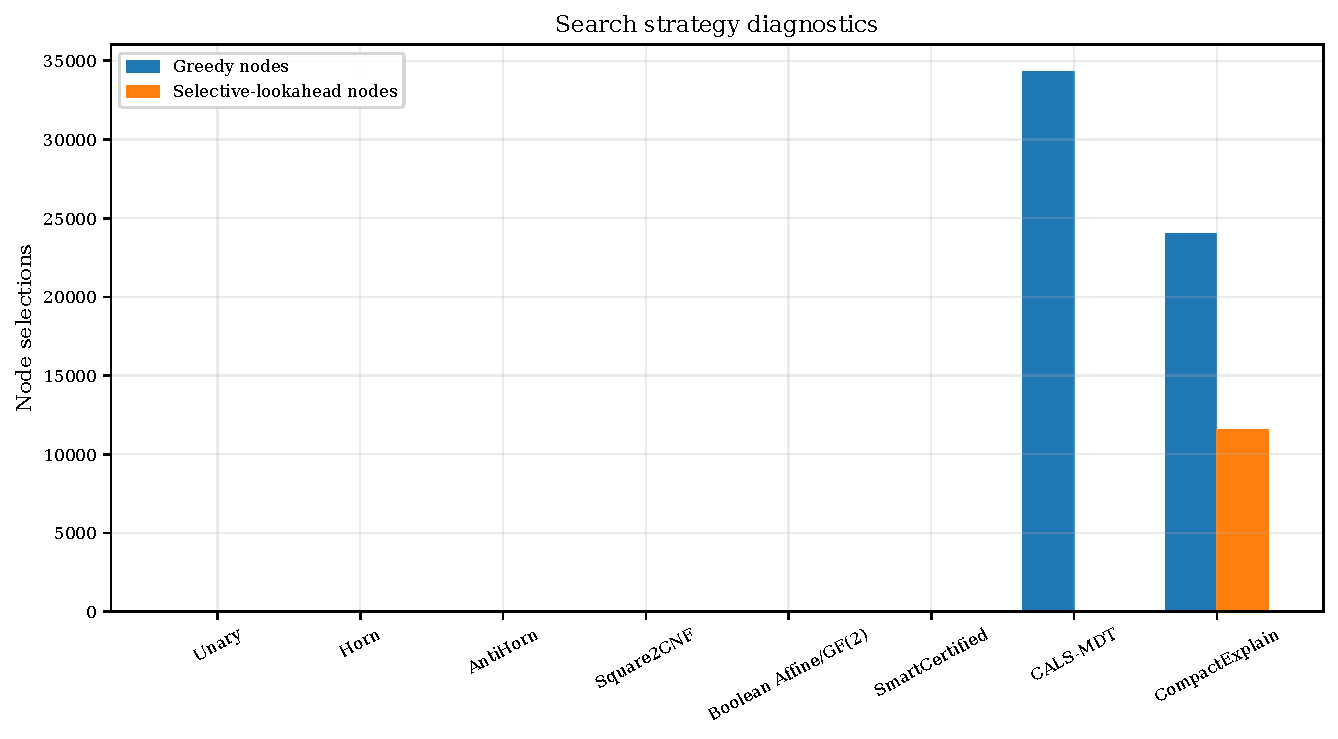
\includegraphics[width=0.82\textwidth]{../figures/search_diagnostics.pdf}
\caption{Greedy and selective-lookahead node selections.}
\end{figure}

\section{Pruning analysis}
\begin{table}[htbp]
\centering
\caption{Validation metrics before and after pruning.}
\label{tab:pruning-validation}
\resizebox{\textwidth}{!}{%
\begin{tabular}{lrrrrrr}
\toprule
Method & Accuracy before & Accuracy after & Balanced before & Balanced after & Minority recall before & Minority recall after \\
\midrule
Unary & 0.000 & 0.000 & 0.000 & 0.000 & 0.000 & 0.000 \\
Horn & 0.000 & 0.000 & 0.000 & 0.000 & 0.000 & 0.000 \\
AntiHorn & 0.000 & 0.000 & 0.000 & 0.000 & 0.000 & 0.000 \\
Square2CNF & 0.000 & 0.000 & 0.000 & 0.000 & 0.000 & 0.000 \\
Boolean Affine/GF(2) & 0.000 & 0.000 & 0.000 & 0.000 & 0.000 & 0.000 \\
SmartCertified & 0.000 & 0.000 & 0.000 & 0.000 & 0.000 & 0.000 \\
CALS-MDT & 0.854 & 0.879 & 0.789 & 0.805 & 0.673 & 0.670 \\
CompactExplain & 0.854 & 0.869 & 0.789 & 0.786 & 0.672 & 0.637 \\
\bottomrule
\end{tabular}%
}
\end{table}

\begin{table}[htbp]
\centering
\caption{Tree-size reduction during pruning.}
\label{tab:pruning-size}
\resizebox{\textwidth}{!}{%
\begin{tabular}{lrrrr}
\toprule
Method & Rows & Nodes before & Nodes after & Tree reduction (\%) \\
\midrule
Unary & 920 & 53.235 & 53.235 & 0.000 \\
Horn & 920 & 51.217 & 51.217 & 0.000 \\
AntiHorn & 920 & 51.487 & 51.487 & 0.000 \\
Square2CNF & 920 & 50.807 & 50.807 & 0.000 \\
Boolean Affine/GF(2) & 920 & 53.126 & 53.126 & 0.000 \\
SmartCertified & 920 & 50.689 & 50.689 & 0.000 \\
CALS-MDT & 920 & 46.133 & 12.730 & 72.405 \\
CompactExplain & 920 & 46.659 & 11.124 & 76.159 \\
\bottomrule
\end{tabular}%
}
\end{table}

\begin{figure}[H]
\centering
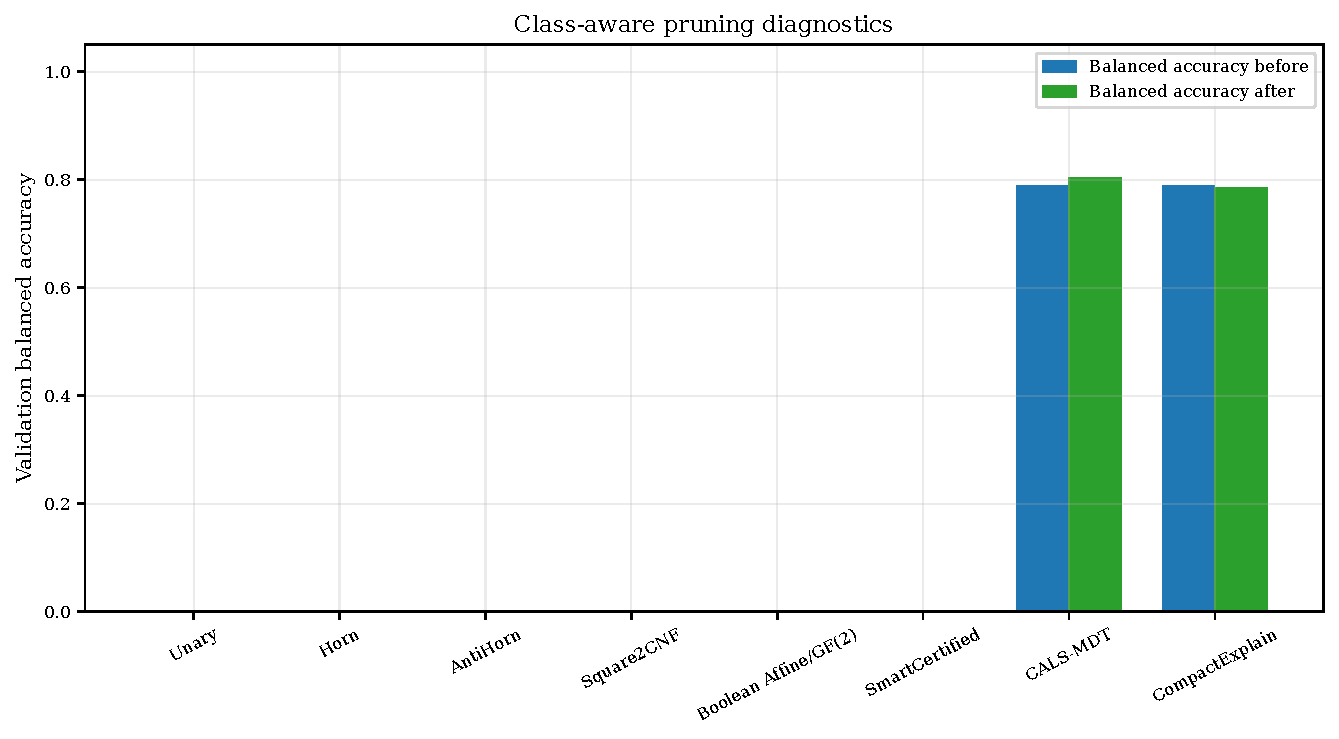
\includegraphics[width=0.82\textwidth]{../figures/pruning_diagnostics.pdf}
\caption{Validation balanced accuracy before and after pruning.}
\end{figure}

\section{AXp analysis}
\begin{table}[htbp]
\centering
\caption{AXp distribution by method.}
\label{tab:axp-distribution}
\resizebox{\textwidth}{!}{%
\begin{tabular}{lrrrrrr}
\toprule
Method & Rows & Mean AXp & Median AXp & AXp std. & Min. AXp & Max. AXp \\
\midrule
Unary & 920 & 3.927 & 3.728 & 1.531 & 0.000 & 9.618 \\
Horn & 920 & 5.137 & 4.887 & 1.892 & 0.000 & 12.863 \\
AntiHorn & 920 & 5.553 & 5.114 & 2.389 & 0.000 & 14.523 \\
Square2CNF & 920 & 6.357 & 5.938 & 2.575 & 0.000 & 17.542 \\
Boolean Affine/GF(2) & 920 & 7.897 & 7.717 & 2.896 & 0.000 & 20.000 \\
SmartCertified & 920 & 4.184 & 3.907 & 1.531 & 0.000 & 10.673 \\
CALS-MDT & 920 & 2.976 & 2.724 & 2.135 & 0.000 & 14.887 \\
CompactExplain & 920 & 2.721 & 2.438 & 2.096 & 0.000 & 15.491 \\
\bottomrule
\end{tabular}%
}
\end{table}

\begin{table}[htbp]
\centering
\caption{Selected predicate-family usage.}
\label{tab:axp-families}
\resizebox{\textwidth}{!}{%
\begin{tabular}{ll}
\toprule
Method & Family usage \\
\midrule
Unary & Unary:24028 \\
Horn & Horn:23100 \\
AntiHorn & AntiHorn:23224 \\
Square2CNF & Square2Cnf:22911 \\
Boolean Affine/GF(2) & Affine:23978 \\
SmartCertified & Affine:1121 | AntiHorn:682 | Horn:2348 | Square2Cnf:150 | Unary:18556 \\
CALS-MDT & Affine:354 | AntiHorn:586 | Horn:1586 | Square2Cnf:1871 | Unary:999 \\
CompactExplain & Affine:281 | AntiHorn:414 | Horn:1063 | Square2Cnf:1720 | Unary:1179 \\
\bottomrule
\end{tabular}%
}
\end{table}


\section{Discussion}
Predictive performance, compactness, runtime, explanation length, and
certification are reported separately. Paired Wilcoxon tests preserve the
dataset blocks after averaging repeated runs and depths. Bootstrap intervals
and effect sizes complement p-values with uncertainty and magnitude. The
generated reproducibility manifest records input hashes, package versions,
seeds, and output files.

\end{document}
